\section{PyGears metodologija} \label{pygears_sec}

\subsection{Uvod}

PyGears\cite{pygears_site} je open-source projekat koji uvodi Gears metodologiju za projektovanje
hardvera i Python Framework koji implementira Gears metodologiju. \\
Gears metodologija uvodi lako povezivanje i kompozabilnost sistema od manjih
funkcionalnih jedinica pod nazivom gear-ovi. \\
Gear moduli su međusobno povezani DTI interfejsom koji implementira jednostavan
handshake protokol.
Na ovaj način je omogućeno je lako ponovno korišćenje implementiranih funkcija i
jednostavno debagovanje dizajna. \\

Pisanjem dizajna u Python-u koji je dinamičan jezik i veoma visokog nivoa
apstrakcije omogućena je dodatno bolje parametrizovanje, skalabilnost i kompozabilnost dizajna. \\

Takođe omogućeno je pisanje verifikacije u Python-u na veoma visokom nivou
apstrakcije uz korišćenje ogromnog broja besplatno dostupnih Python paketa za
većinu problema i algoritama, time je skraćeno vreme i olakšan posao prilikom
pisanja referentnih modela. \\

PyGears konačno obavlja konverziju Python opisa u SystemVerilog opis koji
je podržan od strane alata za sintezi i simulaciju.

\subsection{Poređenje sa RTL metodologijom}

PyGears\cite{PyGears_OSDA} predstavlja alternativu RTL\cite{chu2006rtl} metodologiji za opis hardvera.
RTL metodologija pruža standardan način translacije sekvencijalnog algoritma u
hadverski opis.
Struktura dobijena pomoću RTL metodologije uglavnom se sastoji od \textbf{FSMD}(Finite
State Machine with Datapath). \\
Datapath deo koji sadrži funkcionalne i memorijske jedinice i
mreže za rutiranje podataka\cite{PSDS_5} \\
Mašina stanje koja sadrži registre stanja, logiku za izlazne signale i logiku za
sledeće stanje. \\

Kako dizajn implementiran pomoću RTL metodologije postaje kompleksniji i mašina
stanja postaje kompleksnija i sadrži više stanja.
Pipeline-ovanje, debagovanje  ovakvog dizajna može biti veoma teško. \\
Prednost PyGears metodologije u odnosu na RTL metodologiju najvidljivija je u
sistemima koji su Dataflow orijentisani.

\subsection{Jezici za opis hardvera}

Jezici sa opis hardvera koji se danas daleko najviše koriste su Verilog i VHDL,
nastali su u 1984. i 1983. godine i daleko su siromašniji po mogućnostima od današnjih
jezika višeg nivoa kao što su Python, C++, itd. \\
Najveća prednost ovih jezika je podrška od strane alata za sintezu i simulaciju,
kako se ovi jezici koriste za opis i verifikaciju hardvera preko 30 godina,
alati su zreli i detaljno istestirani. \\

Sve velike kompanije koje proizvode FPGA čipove trenutno ne objavljuju
arhitekturu svojih FPGA čipova, pa alati za sintezu i implementaciju zavise od
tih kompanija\footnote{Postoji inicijativa da se dokumentuju FPGA čipovi svih velikih
proizvođača u projektu zvanom SymbiFlow\cite{SymbiFlow}, kao i alati za sintezu
i implementaciju.}
.
Zbog toga direktna podrška alata za sintezu i implementaciju za neki novi HDL jezik je
nemoguća. \\

Iz tog razloga većina novih HDL jezika baziranih na
Python\cite{decaluwe2004myhdl, PyGears_OSDA}, Scala
\cite{bachrach2012chisel, SpinalHDL}, Haskell\cite{baaij2010c} generišu konačan
HDL kod u Verilog-u, SystemVerilog-u ili VHDL-u pogodnom za simulatore i alate
za sintezu. \\

Dok se ovi jezici uglavnom baziraju na RTL metodologiji i uvode jezik višeg
nivoa kao zamenu za standardan HDL. PyGears dodatno izdvaja i uvođenje nove
metodologije zvane Gears.

\subsection{Gears metodologija}
Cilj Gears metodologije je da se obezbedi bolja kompozabilnost i ponovno
korišćenje napisanih modula. \\
Kako bi se ovo postiglo uveden je standardan interfejs za komunikaciju između
modula.

\subsubsection{DTI interfejs}
\begin{figure}[h]
  \centering
  \includegraphics[width=9cm]{dti}
  \caption{DTI interfejs\cite{PyGears_OSDA}}
  \label{DTI_intf_img}
\end{figure}

Uveden je interfejs \textbf{DTI}(data transfer interface).
Podaci se šalju od strane Producer-a prema Consumer-u.
Sastoji se od:
\begin{itemize}
\item \textbf{Data} linije za podatke, proizvolje širine i proizvoljnog tipa.
\item \textbf{Valid} jednobitnog signala kojim Producer signalizira validnost
  podatka na Data liniji.
\item \textbf{Ready} jednobitnog signala kojim Consumer signalizira da je
  pročitao podatak na Data liniji.
\end{itemize}
Pomoću Valid i Ready signala realizovan je handshaking protokol. \\

\begin{figure}[H]
\centering{
  \scalebox{1.2}{
    \\
\begin{tikztimingtable}[%
    timing/dslope=0.1,
    timing/.style={x=5ex,y=2ex},
    x=5ex,
    timing/rowdist=4ex,
    timing/name/.style={font=\sffamily\scriptsize}
]
\busref{CLK}         & 18{c} \\
\busref{Data}      & 2u 3D 2U 1D 0L 1D 1U \\
\busref{Valid}   & 1L 3H 2L 2H L \\
\busref{Ready} & 3L 5H L  \\
\busref{Event}     & 3U 1D{ACK} 2U 1D{ACK} 1D{ACK} U\\
\extracode
\begin{pgfonlayer}{background}
\begin{scope}[semitransparent ,semithick]
\vertlines[darkgray,dotted]{0.5,1.5 ,...,8.0}
\foreach \i [count=\col from 0] in {0.5,1.5,...,8.0}
    \node[font=\scriptsize] at (\i,3) {${\col}$};
\end{scope}
\end{pgfonlayer}
\end{tikztimingtable}

  }}
\caption{DTI primer transakcije}
\label{dti_example1}
\end{figure}

Na slici(\ref{dti_example1}) prikazan je talasni oblik protokola:
\begin{enumerate}
\item Producer je postavio podatak na Data liniju i podigao Valid signal na
  jedinicu. Što označava validan podatak na magistrali.
\item Istog trenutka nakon postavljanja Valid signala na jedinicu Consumer može
  da koristi podatak na magistrali.
\item Consumer može koristiti podatak na magistrali potreban broj taktova.
\item Kada Consumer završi sa korišćenjem podatka, postavlja Ready signal na
  jedinicu čime označava ACK(acknowledgment) odnosno signalizira da je završio
  sa podatkom na magistrali i da je handshake obavljen. \\
  Nakon handshake-a Producer može postaviti novi podatak na magistralu.
\item Producer ne sme menjati podatak na magistrali sve do pojave ACK od strane
  Consumera.
\item Producer može držati Valid signal na logičkoj nuli i tada se neće
  obavljati transakcije na magistrali.
\item Ne sme postojati kombinaciona putanja od Ready do Valid signala na strani
  Producer-a.
  Odnosno Producer ne sme odlučivati o postavljanju podatka na magistralu na
  osnovu stanja Consumer-a.
\item Može postojati kombinaciona putanja od Valid do Ready signala na strani
  Consumer-a.

\end{enumerate}

\subsection{Tipovi podataka} \label{pygears_data_types}

Data linija u DTI interfejsu pored toga što može biti proizvoljne širine može
predstavljati i različite kompleksne tipove podataka.
Ovim se omogućava bolja kompozicija modula, lakša manipulacija podacima,
pregledniji izvorni kod.

Neki od podržanih tipova su:
\begin{itemize}
\item \textbf{Uint[W]} \ref{uint_sec}
\item \textbf{Int[W]} \ref{int_sec}
\item \textbf{Tuple[T1, T2, ..., TN]} \ref{tuple_sec}
\item \textbf{Array[T, N]} \ref{array_sec}
\item \textbf{Queue[T, LVL]} \ref{queue_sec}
\item \textbf{Union[T1, T2, ..., TN]} \ref{union_sec}
\item \textbf{Unit} \ref{unit_sec}
\end{itemize}

\subsubsection{Uint} \label{uint_sec}
\textbf{Uint[W]} predstavlja neoznačenu celobrojnu vrednost proizvoljne
širine W.

\subsubsection{Int} \label{int_sec}
\textbf{Int[W]} predstavlja označenu celobrojnu vrednost proizvoljne
  širine W.

\subsubsection{Tuple} \label{tuple_sec}
\textbf{Tuple[T1, T2, ..., TN]} predstavlja tip sličan strukturi gde
  polja Tn mogu biti bilo kog tipa. \\
  Koordinate piksela slike mogu se prigodno predstaviti kao Tuple tip. \\
  Na primer Tuple[Uint[W\_Y], Uint[W\_X]] ovaj Tuple sadrži dva Uint polja koji
  predstavljaju X i Y koordinate.

\subsubsection{Array} \label{array_sec}
\textbf{Array[T, N]} predstavlja niz od N podataka tipa T.

\subsubsection{Queue} \label{queue_sec}
\textbf{Queue[T, LVL]} ili red predstavlja transakciju koja sadrži više
  podataka proizvoljnog tipa T i informaciju o završetku transakcije EOT(end of
  transaction).
  Queue može biti proizvoljnog nivoa LVL. \\
  Kao primer \textbf{Queue[Uint[4], 1](0, 1, 2, 3)} predstavlja red od četiri
  četvorobitna podatka.
  Rezultujuća Data magistrala biće širine 5 bita, 4 bita za podatak i 1 bit za EOT.
\begin{figure}[H]
\centering{
  \scalebox{1.2}{
    \\
\begin{tikztimingtable}[%
    timing/dslope=0.1,
    timing/.style={x=5ex,y=2ex},
    x=5ex,
    timing/rowdist=4ex,
    timing/name/.style={font=\sffamily\scriptsize}
]
\busref{CLK}         & 12{c} \\
\busref{Data}[4:0]      & 2u 1D{0x00} 1D{0x01} 1D{0x02} 1 D{0x13}  U \\
\busref{Data[3:0]} & 2u 1D{0} 1D{1} 1D{2} 1D{3} U \\
\busref{EOT\textsubscript{(Data[4])}} & U 3L 1H U \\
\busref{Valid}   & 1L 4H L \\
\busref{Ready} & 4L 1H L  \\
\busref{Event}     & 4U 1D{ACK} U \\
\extracode
\begin{pgfonlayer}{background}
\begin{scope}[semitransparent ,semithick]
\vertlines[darkgray,dotted]{0.5,1.5 ,...,6.0}
\foreach \i [count=\col from 0] in {0.5,1.5,...,6.0}
    \node[font=\scriptsize] at (\i,3) {${\col}$};
\end{scope}
\end{pgfonlayer}
\end{tikztimingtable}
  }}
\caption{Primer transakcije tipa}
\label{queue_img1}
\end{figure}

Kao primer dvodimenzionalna matrica se može predstaviti kao Queue[Uint[4], 2],
odnosno red nivoa 2 sa proizvoljnim podatkom u ovom slučajem četvorobitnim
neoznačnim brojem.

\begin{figure}[H]
\centering{
  \scalebox{0.9}{
    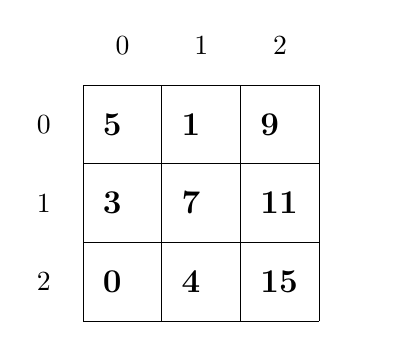
\begin{tikzpicture}
  % draw the grid and the numbers
  \draw (-1,-1) grid (2,2) foreach \i in {0,...,2}{
    (\i-.5,2.5) node{\i} (-1.5,1.5-\i) node{\i}};

  \node[text width=1.5cm] at (0.0,1.5) (A_coord) {\large \textbf{5}};
  \node[text width=1.5cm] at (1.0,1.5) (A_coord) {\large \textbf{1}};
  \node[text width=1.5cm] at (2.0,1.5) (A_coord) {\large \textbf{9}};

  \node[text width=1.5cm] at (0.0,0.5) (A_coord) {\large \textbf{3}};
  \node[text width=1.5cm] at (1.0,0.5) (A_coord) {\large \textbf{7}};
  \node[text width=1.5cm] at (2.0,0.5) (A_coord) {\large \textbf{11}};

  \node[text width=1.5cm] at (0.0,-0.5) (A_coord) {\large \textbf{0}};
  \node[text width=1.5cm] at (1.0,-0.5) (A_coord) {\large \textbf{4}};
  \node[text width=1.5cm] at (2.0,-0.5) (A_coord) {\large \textbf{15}};

\end{tikzpicture}

  }}
\caption{Matrice veličine 3x3}
\label{queue_matrix1}
\end{figure}

\begin{figure}[H]
\centering{
  \scalebox{1.2}{
    \\
\begin{tikztimingtable}[%
    timing/dslope=0.1,
    timing/.style={x=5ex,y=2ex},
    x=5ex,
    timing/rowdist=4ex,
    timing/name/.style={font=\sffamily\scriptsize}
]
\busref{CLK}         & 22{c} \\
\busref{Data}[5:0]      & 2u 1D{0x05} 1D{0x01} 1D{0x19} 1D{0x03} 1D{0x07}
1D{0x1B} 1D{0x00} 1D{0x04} 1D{0x1F} U \\
\busref{Data[3:0]} & 2u 1D{5} 1D{1} 1D{9} 1D{3} 1D{7} 1D{11} 1D{0} 1D{4} 1D{15}  U \\
\busref{EOT[1]\textsubscript{(Data[5])}} & U 6L 3H U \\
\busref{EOT[0]\textsubscript{(Data[4])}} & U 2L 1H 2L 1H 2L 1H U \\
\busref{Valid}   & 1L 9H L \\
\busref{Ready} & 9L 1H L  \\
\busref{Event}     & 9U 1D{ACK} U \\
\extracode
\begin{pgfonlayer}{background}
\begin{scope}[semitransparent ,semithick]
\vertlines[darkgray,dotted]{0.5,1.5 ,...,11.0}
\foreach \i [count=\col from 0] in {0.5,1.5,...,11.0}
    \node[font=\scriptsize] at (\i,3) {${\col}$};
\end{scope}
\end{pgfonlayer}
\end{tikztimingtable}

  }}
\caption{Transakcija matrice \ref{queue_matrix1}}
\label{queue_matrix2}
\end{figure}

Kao što se može videti linija za podatke je u ovom slučaju širine 6 bita, od
toga 2 bita su EOT. \\
Na slici(\ref{queue_matrix1}) u taktovima(3, 6, 9) niži bit EOT-a je na visokom nivou
što predstavlja podatak u poslednjoj koloni matrice.
U taktovima(7, 8, 9) viši bit EOT-a je na visokom nivou što označava podatke u poslednjoj
liniji matrice.
Konačno u taktu 9 oba EOT bita su na visokom nivou što označava poslednji podatak u matrici.

\subsubsection{Union} \label{union_sec}
\textbf{Union[T1, T2, ..., TN]} je unija koja može prenositi samo jedan od
  podataka Tn u trenutku.
  Uz podatak prenosi se i informacija o aktivnom podatku na magistrali.

\subsubsection{Unit} \label{unit_sec}
\textbf{Unit} je tip koji ne prenosi podatak.

\begin{figure}[H]
\centering{
  \scalebox{1.2}{
    \\
\begin{tikztimingtable}[%
    timing/dslope=0.1,
    timing/.style={x=5ex,y=2ex},
    x=5ex,
    timing/rowdist=4ex,
    timing/name/.style={font=\sffamily\scriptsize}
]
\busref{CLK}         & 6{c} \\
\busref{Valid}   & 1L 1H L \\
\busref{Ready} & 1L 1H L  \\
\busref{Event}     & 1U 1D{ACK} U \\
\extracode
\begin{pgfonlayer}{background}
\begin{scope}[semitransparent ,semithick]
\vertlines[darkgray,dotted]{0.5,1.5 ,...,3.0}
\foreach \i [count=\col from 0] in {0.5,1.5,...,3.0}
    \node[font=\scriptsize] at (\i,3) {${\col}$};
\end{scope}
\end{pgfonlayer}
\end{tikztimingtable}
  }}
\caption{Unit tip}
\label{unit_img1}
\end{figure}

\subsection{Čistoća Gear-ova} \label{gear_purity}

Kako bi se gear-ovi lakše povezivali i njihova funkcionalnost i ponašanje bilo
razumljivo i predvidljivo dizajneru preporučuje se pisanje ``Čistih''  gear-ova. \\
``Čist'' gear je onaj čije je inicijalno stanje dobro poznato i koji će se nakon
izvršene funkcionalnosti potpuno vratiti u inicijalno stanje. \\
Čisto kombinacioni gear-ovi su uvek ``čisti''.

\subsection{Definicija Gear komponenti}

PyGears trenutno podržava tri načina za implementaciju Gear komponenti.

\lstinputlisting[language=Python, mathescape, caption={Primer definisanja Gear
  komponente}, captionpos=b, label=gear_example1]{gear1.py}

Primer(\ref{gear_example1}) prikazuje definisanje gear komponente. \\
Dekorator \textbf{@gear} označava da je funkcija gear\_name zapravo Gear komponenta,
slično kao module ili entity kod Verilog-a i VHDL-a. \\
Kao parametri funkcije prosleđuju se DTI interfejsi i generički parametri.
Delimiter ``*'' označava početak generičkih parametara. \\

Ulazni DTI interfejsi mogu imati proizvoljan naziv i tipove opisane u
sekciji(\ref{pygears_data_types}). \\
Parametar može biti bilo koji Python objekat i može imati inicijalnu vrednost dflt.

\subsubsection{Gear implementiran pomoću SystemVerilog-a}

Jedan od mogućih načina implementacije Gear komponente je pisanje SystemVerilog
opisa pa zatim Python wrapper-a za komponentu. \\
Prilikom pisanja modula na ovaj način potrebno je pobrinuti se da dobijena
komponenta poštuje DTI protokol kao i da je ``čist'' Gear(\ref{gear_purity}). \\

Prilikom pisanja wrapper-a za ovako implementiranu komponentu potrebno je
unapred odrediti ReturnType koji će odgovarati izlaznom interfejsu SystemVerilog modula. \\
Takođe deo za implementaciju Gear-a u Python-u može ostati prazan. \\

Kako postoji velika verovatnoća unošenja bagova u dizajn prilikom ručnog pisanja
modula koji poštuje DTI interfejs i koji je ``čist'', ovaj način implementacije
modula nije preporučen.

\subsubsection{Gear implementiram kompozicijom}

Kako PyGears dolazi sa bibliotekom osnovnih funkcionalnih modula, većina
potrebnih funkcionalnosti moguće je ostvariti njihovom kompozicijom. \\

\subsubsection{Gear implementiram Python to HDL kompajlerom}

Kako PyGears dolazi sa bibliotekom osnovnih funkcionalnih modula, većina
potrebnih funkcionalnosti moguće je ostvariti njihovom kompozicijom. \\